
\chapter{Theoretical background} 
\label{ch:THback}

In this chapter, we will present the theory upon which this work is based. First, the light propagation formalism will be reminded through the scalar diffraction theory based on the \citet{goodman_1968}. Then we will describe in general an imaging system and its properties. And finally we will discuss the wavefront aberration theory.

\section{Scalar Diffraction Theory}
\label{sec:ScaDifTh}

\subsection{Scalar Field and Helmholtz equation}
\label{subsec:ScalF_HelmEqt}

A monochromatic wave, at position $P$ and time $t$, can be represented by a scalar field $u(P,t)$ written as :

\begin{equation}
u(P,t) =  A(P) exp\left[-j2\pi\nu t - j\phi(P)\right],
\label{eqt:WvscalarField}
\end{equation}

where $A(P)$ and $\phi(P)$ are the amplitude and phase, respectively, of the wave at position P and $\nu$ is the wave frequency.

The spatial part of eqt. \eqref{eqt:WvscalarField}, also called  phasor  in the literature, 

\begin{equation}
U(P) = A(P)e^{-j\phi(P)},
\label{eqt:phasor}
\end{equation}

must verify the Helmotz equation : 

\begin{equation}
(\nabla^2 + k^2)U = 0,
\label{eqt:HelmholtzEqt}
\end{equation}

where $k$ is the wave number given by

\begin{equation}
k = 2\pi n \frac{\nu}{c} = \frac{2\pi}{\lambda},
\label{eqt:wavenumber}
\end{equation}

and $\lambda$ is the wavelength in the dielectric medium.


\subsection{Rayleigh-Sommerfeld integral}
\label{subsec:Ray_Som_int}

\begin{figure}
\centering
    \begin{subfigure}{0.4\textwidth}
        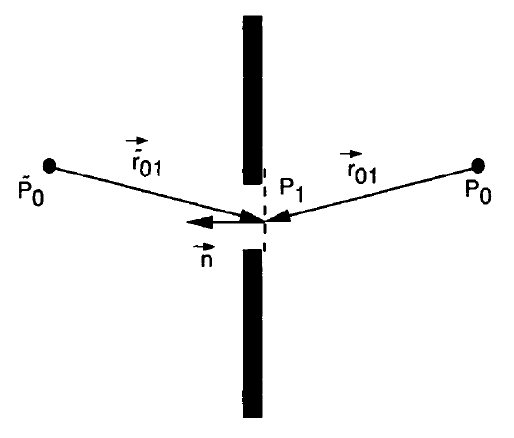
\includegraphics[width=\textwidth]{Figures/Ray_Som_Diff}
        \caption{Rayleigh-Sommerfeld formulation of diffraction by a plane screen, \citep[Chapter 3.5]{goodman_1968}.}
        \label{subfig:Ray_Som_Diff}
    \end{subfigure}
    \quad
    \begin{subfigure}{0.5\textwidth}
        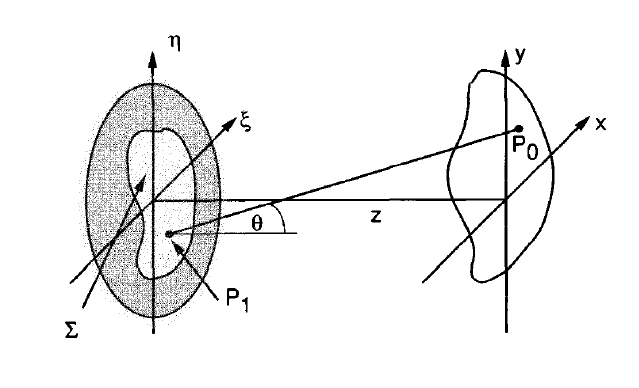
\includegraphics[width=\textwidth]{Figures/Diff_Geom}
        \caption{Diffraction geometry, \citep[Chapter 4.1]{goodman_1968}.}
        \label{subfig:Diff_Geom}
    \end{subfigure}
    \decoRule
    \caption{Diffraction Schemas}
    \label{fig:Diff_Schemas}
\end{figure}

Rayleigh and Sommerfeld developed a formalism using the Helmholtz equation and Green's Theorem to compute the induced diffraction by a plane screen. Let's suppose that we have a monochromatic source at $\widetilde{P_0}$ on the left of a plane screen with aperture $\Sigma$, the Rayleigh-Sommerfeld formula allows to compute the complex amplitude at $P_0$ on the right of the plane screen (see Figure \ref{subfig:Ray_Som_Diff}).

\begin{equation}
U(P_0) = \frac{1}{j\lambda} \iint\limits_{\Sigma} U'(P_1)\frac{exp(jkr_{01})}{r_{01}}cos(\mathbf{n},\mathbf{r_{01}})\mathbf{ds}
\label{eqt:Ray_Som_Formula}
\end{equation}

$U'(P_1)$ is the complex amplitude on the screen, $cos(\mathbf{n},\mathbf{r_{01}})$ is the cosine of the angle between the aperture plane normal toward the source and the vector $\mathbf{r_{01}} = \mathbf{P_0P_1}$ given by 

\begin{equation}
r_{01} = \sqrt{z^2 + (x-\xi)^2 + (y-\eta)^2}.
\label{eqt:r_01}
\end{equation}

We can rewrite eqt. \eqref{eqt:Ray_Som_Formula} using $cos(\mathbf{n},\mathbf{r_{01}}) = cos(\theta) = \frac{z}{r_{01}}$ and the coordinate systems ($\xi,\eta$) and ($x,y$), see Figure \ref{subfig:Diff_Geom},

\begin{equation}
U(x,y) = \frac{z}{j\lambda} \iint\limits_{-\infty}^{\infty} U(\xi,\eta)\frac{exp(jkr_{01})}{r_{01}^2} d\xi d\eta.
\label{eqt:Ray_Som_formula_xy_en}
\end{equation}

We can integrate from $-\infty$ to $\infty$, using $U(\xi,\eta) = P(\xi,\eta)U'(\xi,\eta)$ where $P(\xi,\eta)$ is the pupil function. The latter equals to one in the pupil and zero outside. 

\subsection{Fresnel approximation}
\label{subsec:FresnelApprox}

To reduce eqt. \eqref{eqt:Ray_Som_formula_xy_en}, also known as the Huygens-Fresnel principle, one can approximate the distance $r_{01}$ using the taylor expansion of the square root :

\begin{equation}
r_{01} = z \sqrt{1 + \frac{x-\xi}{z} + \frac{y-\eta}{z}} \approx z \left[1+\frac{1}{2}\left(\frac{x-\xi}{z}\right)^2+\frac{1}{2}\left(\frac{y-\eta}{z}\right)^2\right]
\label{eqt:approx_r01}
\end{equation}

To obtain the Fresnel approximation, one has to replace $r_{01}$ by eqt. \eqref{eqt:approx_r01} in eqt. \eqref{eqt:Ray_Som_formula_xy_en}. At the denominator, only the first term $z$ is kept, since the introduced error is small, but in the exponential everything is kept. Then the final expression is given by,

\begin{equation}
U(x,y) = \frac{e^{jkz}}{j\lambda z} \iint\limits_{-\infty}^{\infty} U(\xi,\eta)exp \left\lbrace j \frac{k}{2z}\left[(x-\xi)^2+(y-\eta)^2\right]\right\rbrace d\xi d\eta.
\label{eqt:fresnel_Approx_conv}
\end{equation}

In this form, the Fresnel approximation can be seen as a convolution between $U(\xi,\eta)$ and $h(x,y) = \frac{e^{jkz}}{j\lambda z}exp\left[\frac{jk}{2z}\left(x^2+y^2\right)\right]$.

Another form is found by developing $\left[(x-\xi)^2+(y-\eta)^2\right]$,

\begin{equation}
U(x,y) = \frac{e^{jkz}}{j\lambda z} e^{j\frac{k}{2z}(x^2+y^2)} \iint\limits_{-\infty}^{\infty} \left\lbrace U(\xi,\eta) e^{j\frac{k}{2z}(\xi^2+\eta^2)}\right\rbrace e^{-j\frac{2\pi}{\lambda z}(x\xi+y\eta)} d\xi d\eta,
\label{eqt:fresnel_Approx_FT}
\end{equation}

it is the Fourier transform of the complex field in the pupil multiplied by a quadratic phase exponential.

\subsection{Fraunhofer approximation}
\label{subsec:FraunhoferApprox}

In addition to the Fresnel approximation, we can introduce another approximation using the condition,

\begin{equation}
z >> \frac{k(\xi^2+\eta^2)_{max}}{2}.
\label{eqt:Fraun_Cond}
\end{equation}

If eqt. \eqref{eqt:Fraun_Cond} is satisfied the Fresnel approximation simplifies, since the quadratic phase factor in $(\xi,\eta)$ is approximately one on the entire pupil, as

\begin{equation}
U(x,y) = \frac{e^{jkz}}{j\lambda z} e^{j\frac{k}{2z}(x^2+y^2)} \iint\limits_{-\infty}^{\infty} U(\xi,\eta) e^{-j\frac{2\pi}{\lambda z}(x\xi+y\eta)} d\xi d\eta.
\label{eqt:Fraunhofer_approx}  
\end{equation}

For instance, at a wavelength of 637.5 nm and a pupil diameter of 3.6 mm the Fraunhofer approximation constrain $z$ to be greater than 63 meters to be valid.

\subsection{Converging lens introduction}
\label{subsec:ConvLensIntro}

The Fraunhofer conditions are severe as shown above, but one can reduce the distance $z$ by observing at the focal plane of a converging lens. Indeed, using the paraxial approximation, i.e. small angles with respect with the optical axis, the lens transmission function is given by,

\begin{align}
t_l(\xi , \eta) &= exp \left[ j k n \Delta_0 \right] exp \left[ -jk \left( n-1 \right)\frac{ \xi^2 + \eta^2 }{2}\left( \frac{1}{R_1} - \frac{1}{R_2}\right) \right] \nonumber \\ 
&= exp \left[ -j \frac{k}{2f} (\xi^2+\eta^2) \right] ,
\label{eqt:lensTl}
\end{align}

where $n$ is the refractive index of the lens material, $R_1$ and $R_2$ are the radii of curvature of the front and back surface of the lens, respectively and f is the focal length of the lens defined as,

\begin{equation}
\frac{1}{f} \equiv (n-1)\left(\frac{1}{R_1}-\frac{1}{R_2}. \right)
\label{eqt:focal_length}
\end{equation}

We can define $U_l(\xi,\eta) = U(\xi,\eta)t_l(\xi,\eta)$, which represents the complex amplitude passing through a lens. Finally, replacing $U(\xi,\eta)$ by $U_l(\xi,\eta)$ in Fresnel approximation and setting the observing distance to the focal length of the converging lens, we recover the Fraunhofer approximation,

\begin{align}
U(x,y) &= \frac{e^{jkz}}{j\lambda z} e^{j\frac{k}{2z}(x^2+y^2)}  \mathcal{F}\left\lbrace U(\xi,\eta) exp\left[j\frac{k}{2}(\xi^2+\eta^2)(\frac{1}{z}-\frac{1}{f})\right]\right\rbrace \nonumber \\
&\overset{z=f}{=} \frac{e^{jkz}}{j\lambda z} e^{j\frac{k}{2z}(x^2+y^2)}  \mathcal{F}\left\lbrace U(\xi,\eta)\right\rbrace.
\end{align}

\section{Imaging system}
\label{sec:ImSystem}

\begin{figure}
\begin{center}
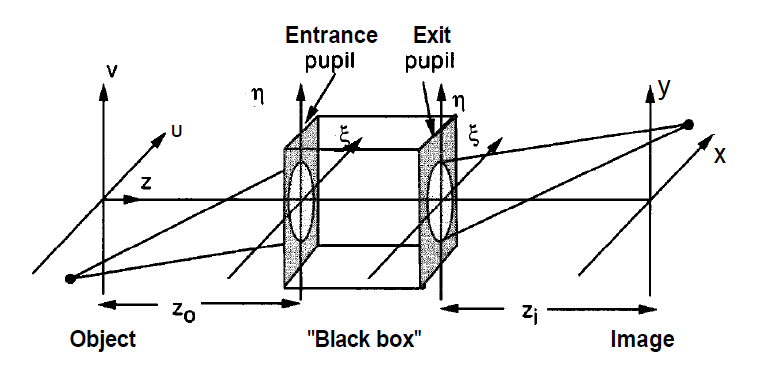
\includegraphics[width=0.8\textwidth,angle=0]{Figures/ImagingInstrumentGenSchema}
\decoRule
\caption{Schema of a imaging instrument, \citep[Chapter 6.1]{goodman_1968}}
\label{fig:ImagingInstrumentGenSchema}
\end{center}
\end{figure}

An imaging system, such as a telescope, is used to acquire images of an object as perfectly as possible. An optical system,  forming an instrument, is composed by lenses, mirrors, etc... and a detector (can be the human eye). A complex optical system can be reduced to a pupil, $P(\xi,\eta)$, and a focal length, $f$. The diffraction of the wave can be determined by the Fraunhofer approximation as long as the paraxial approximation is valid, see subsection \ref{subsec:ConvLensIntro}. And the observed image of an incoherent object at the focal plane of the system is proportional to the square modulus of the complex amplitude $U(x,y)$,

%\begin{equation}
%i(x,y) \alpha |\left[\mathcal{F}\left\lbrace U(\xi,\eta) \right\rbrace\right](x,y)|^2.
%\label{eqt:i_modu_FT}
%\end{equation}

\subsection{Impulse Response (IR)}
\label{subsec:IR} 

The impulse response or point spread function (PSF), $h(x,y;u,v)$, of an optical system is  the field amplitude induced at coordinates $(x,y)$ by a unit-amplitude point source at object coordinates $(u,v)$. Using the linearity of the wave propagation, we can write the imaged amplitude as a superposition integral,

\begin{equation}
U(x,y) = \iint_{-\infty}^{\infty} h(x,y;u,v)U(u,v)dudv
\label{eqt:superpositionIntegral}
\end{equation}

\subsection{Optical Transfer Function (OTF)}
\label{subsec:OTF}

\begin{figure}
\begin{center}
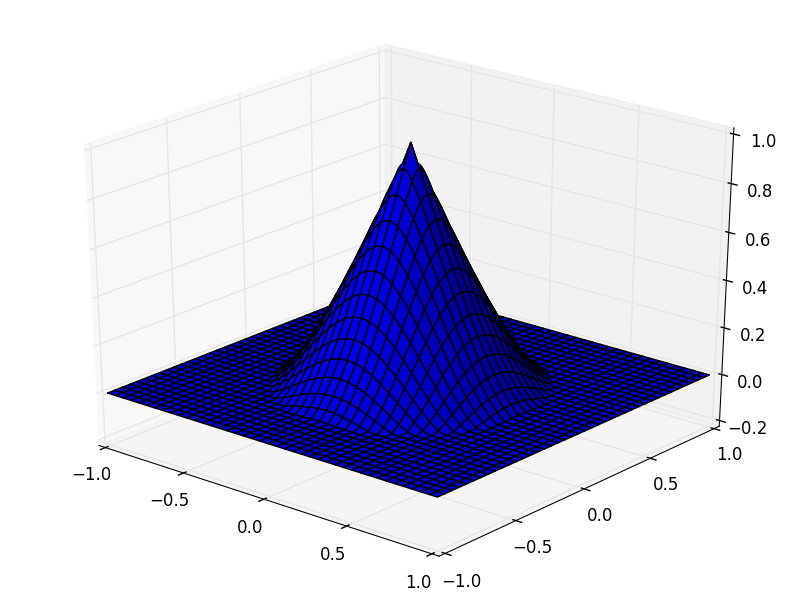
\includegraphics[width=0.5\textwidth,angle=0]{Figures/OTF}
\decoRule
\caption{OTF of a perfect imaging system composed by a 3.6 mm pupil and a focal length of 80 mm at a wavelength of 637.5 nm.}
\label{fig:OTF}
\end{center}
\end{figure}

The optical transfer function, OTF, is defined as the Fourier transform of the impulse response, an example is shown in Figure \ref{fig:OTF}. As we will use it later, for incoherent illumination and using the Fourier transform properties it can also be given by the autocorrelation of the pupil function as we will see in section \ref{subsec:FromOtoI} that the impulse response is given by the Fourier transform of the squared pupil function,

\begin{equation}
\widetilde{h}_{optical}(\xi,\eta) = \mathcal{F}\left\lbrace h_{optical}(x,y)\right\rbrace = (P \otimes P)(\xi,\eta),
\label{eqt:OTF}
\end{equation}

where $\xi$ and $\eta$ are the conjugate variables of $x$ and $y$ with respect to the Fourier transform.

\subsection{From Object to Image}
\label{subsec:FromOtoI}

A detector only senses the energy distribution produced by an electromagnetic wave. Therefore, an image is given by the square modulus of the complex amplitude at the focal plane,

\begin{equation}
i(x,y) = |U(x,y)|^2 = |\iint_{-\infty}^{\infty} h(x,y;u,v)U(u,v)dudv|^2.
\label{eqt:IsqAmplitude}
\end{equation}

This integral simplifies differently depending on the type of object we are observing. For a \textbf{coherent object}, \citet[Chapter 6.2]{goodman_1968} showed that the imaging is linear in complex amplitude, thus eqt. \eqref{eqt:IsqAmplitude} becomes,

\begin{equation}
i(x,y) = |\iint_{-\infty}^{\infty} h(x-\widetilde{u},y-\widetilde{v})U(\widetilde{u},\widetilde{v})d\widetilde{u}d\widetilde{v}|^2,
\label{eqt:convolution_hUo}
\end{equation}

where $(\widetilde{u} = Mu,\widetilde{v}= Mv)$ are the normalized object coordinates and $M$ is the magnification of the imaging system. The image is given by the squared modulus of the convolution of the impulse response and the object complex amplitude.

For an \textbf{incoherent object},  \citet[Chapter 6.2]{goodman_1968} showed that the imaging is linear in intensity,

\begin{equation}
i(x,y) = \iint_{-\infty}^{\infty}|h(x-\widetilde{u},y-\widetilde{v})|^2o(\widetilde{u},\widetilde{v})d\widetilde{u}d\widetilde{v} = (h_{optical}\otimes o)(x,y),
\label{eqt:imageObjectrel}
\end{equation}

where $o(x,y) = |U(x,y)|^2$. We can recognize the convolution of an object with an intensity impulse response, $h_{optical}(x,y) = |h(x,y)|^2$.

\begin{figure}
\centering
    \begin{subfigure}{0.45\textwidth}
        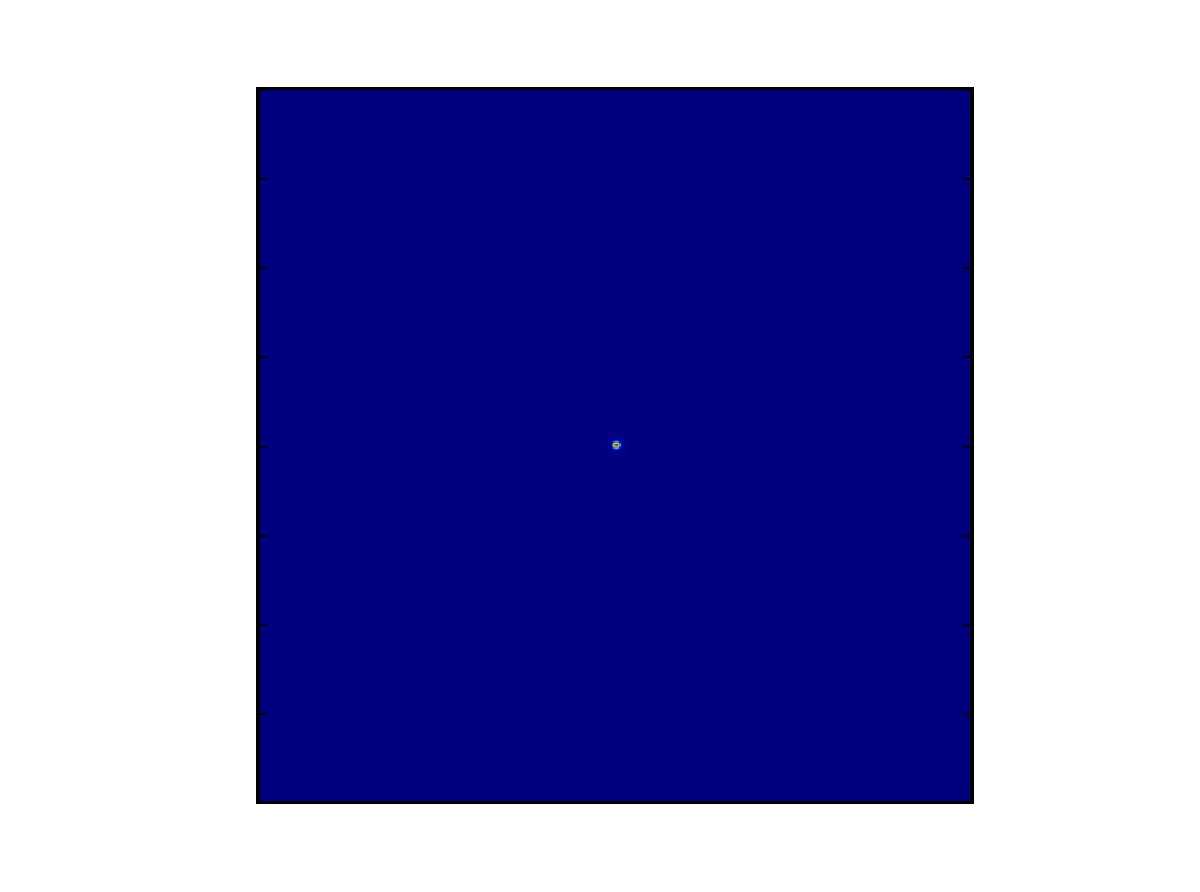
\includegraphics[width=\textwidth]{Figures/PSF}
        \caption{PSF}
        \label{subfig:PSF}
    \end{subfigure}
    \quad
    \begin{subfigure}{0.45\textwidth}
        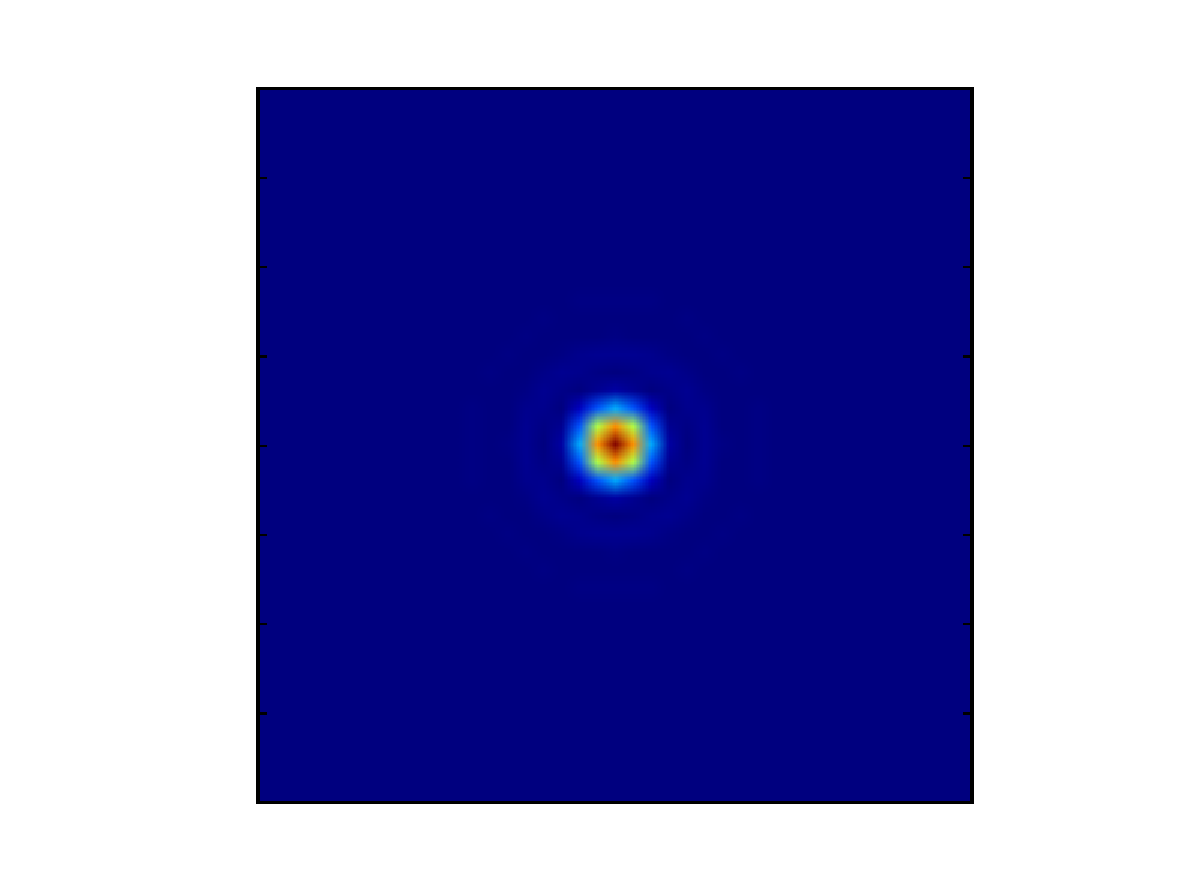
\includegraphics[width=\textwidth]{Figures/PSFzoom}
        \caption{PSF zoom x10}
        \label{subfig:PSFzoom}
    \end{subfigure}
    \decoRule
    \caption{PSF of a perfect imaging system composed by a 3.6 mm pupil and a focal length of 80 mm at a wavelength of 637.5 nm. The size, N, of the PSF is 400 and the pixel size is 5.3 $\mu m$.}
    \label{fig:PSF}
\end{figure}

In this study, we will study stars radiation which are object with an incoherent emission. The stars are point source objects given there distances. The image that an optical system gives of a point source is called the point spread function, PSF, or impulse response, IR, of the system, see Figure \ref{fig:PSF}. A point source is characterized by an infinite distance to the instrument and therefore the wave is planar, which means that the phasor is reduced to $U(\xi,\eta) = P(\xi,\eta)$. The PSF or IR is given by,

\begin{equation}
h_{optical}(x,y) = |\left[\mathcal{F}\left\lbrace P(\xi,\eta) \right\rbrace\right](x,y)|^2
\label{eqt:impulseResponse}
\end{equation}

The domain where the impulse response is invariant under translation is called the \textbf{isoplanatic domain}.

In presence of aberrations, which will be discussed in section \ref{sec:Aberrations}, the wavefront is deformed with respect to the perfect planar or spheric form. The pupil function at the exit of the imaging system is modified as following,

\begin{equation}
\mathcal{P}(\xi,\eta) = P(\xi,\eta) e^{-j\phi_{Ab}(\xi,\eta)},
\label{eqt:aberratedPhasor}
\end{equation}

where $\phi_{Ab}(\xi,\eta)$ is the dephasing caused by the aberration present between the object and the image planes. Replacing the new pupil function in eqt. \eqref{eqt:impulseResponse}, we obtain the PSF of an imaging system having aberrations on the optical path.

\section{Aberrations}
\label{sec:Aberrations}

\begin{minipage}{\linewidth}
\begin{wrapfigure}{r}{0.5\textwidth}
\centering
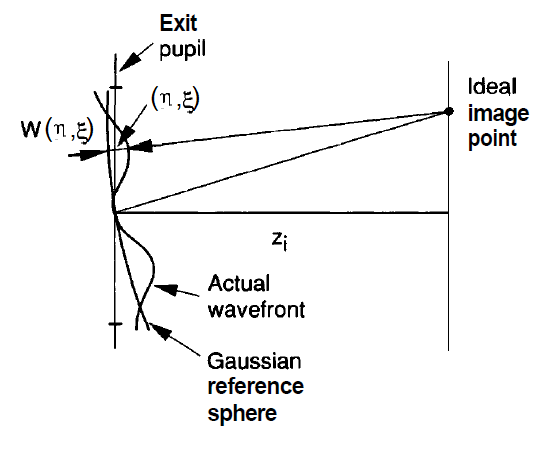
\includegraphics[width=0.5\textwidth]{Figures/AbWFvsGausSphWF}
\decoRulewrapFig
\caption[Gaussian reference sphere vs. aberrated Wavefront]{Gaussian reference sphere vs. aberrated Wavefront, \citep[Chapter 6.4]{goodman_1968}. The dephasing is equal to the wave number multiplied by the aberration function, $\phi_{Ab}(\xi,\eta) = k W(\xi,\eta)$.}
\label{fig:AbWFvsGausSphWF}
\end{wrapfigure}

The aberrations present on the optical path between the object and the image planes decrease the quality of the resulting image. Indeed, they induce fluctuations of the amplitude and phase of the wave in the pupil plane. Since the amplitude fluctuations are negligible with respect to the phase fluctuations, we focus only on the latter. In figure \ref{fig:AbWFvsGausSphWF}, one can see the effect of the aberrations on an hypothetical spherical wavefront at the exit pupil of an imaging system. And in Figure \ref{fig:ComparisonPSFs}, one can see the effect of aberrations on the PSF of an imaging system. The PSF is blurred due to the defocus and we can well recognize the astigmatism introduced as the shape of the PSF tends towards the ellipse. The Strehl ratio is often the used quantity to quantify the importance of the aberrations, it is given by the following expression,

\begin{equation}
SR = \frac{\int \widetilde{h}_{optical}(\xi,\eta)\mathrm{d}\xi \mathrm{d}\eta}{\int \widetilde{h}_{perfect}(\xi,\eta) \mathrm{d}\xi \mathrm{d}\eta},
\label{eqt:StrehlRatio}
\end{equation}

where $\widetilde{h}_{perfect}(\xi,\eta)$ it the OTF of the perfect system with the same pupil as the optical system with the OTF $\overset{\sim}{h}_{optical}(\xi,\eta)$.
\end{minipage}

\begin{figure}
 \centering
     \begin{subfigure}{0.45\textwidth}
         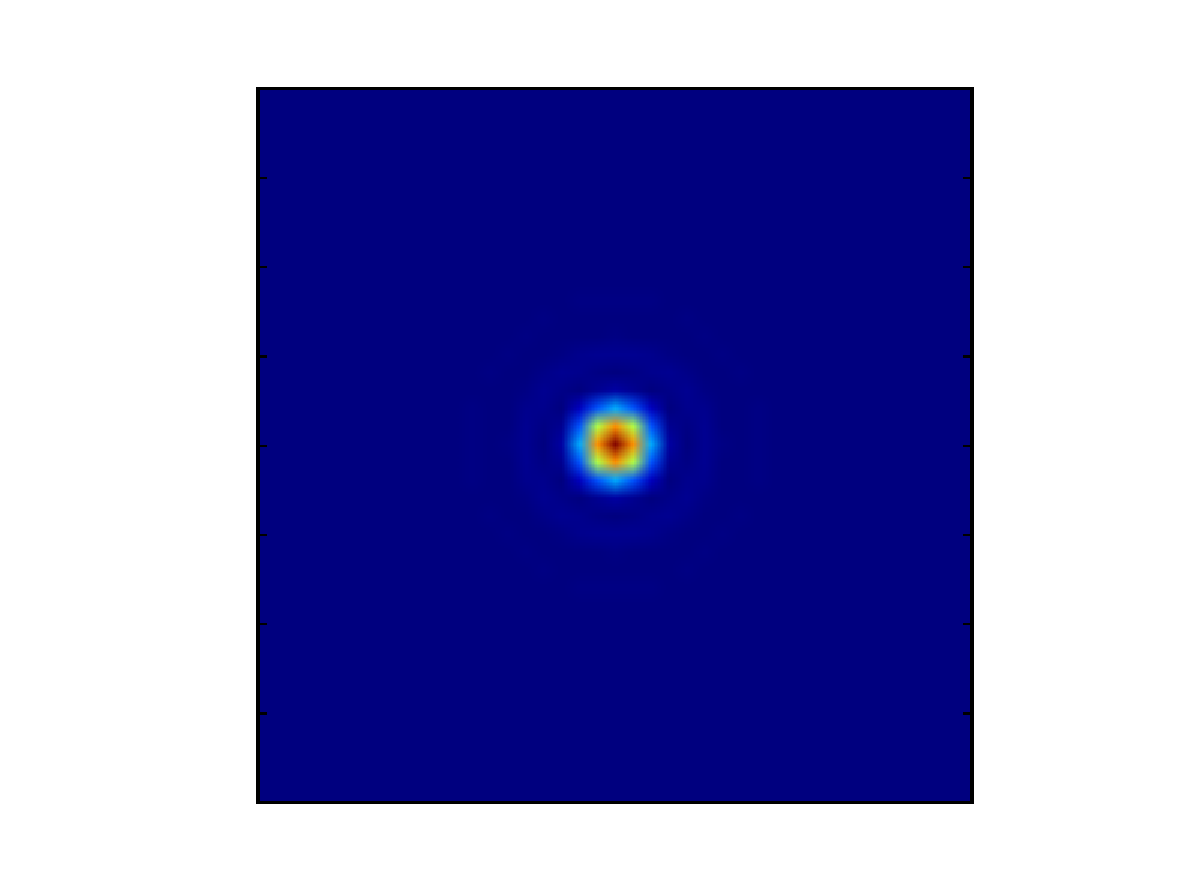
\includegraphics[width=\textwidth]{Figures/PSFzoom}
         \caption{perfect PSF (zoomed x10)}
         \label{subfig:perfPSF}
     \end{subfigure}
     \quad
     \begin{subfigure}{0.45\textwidth}
         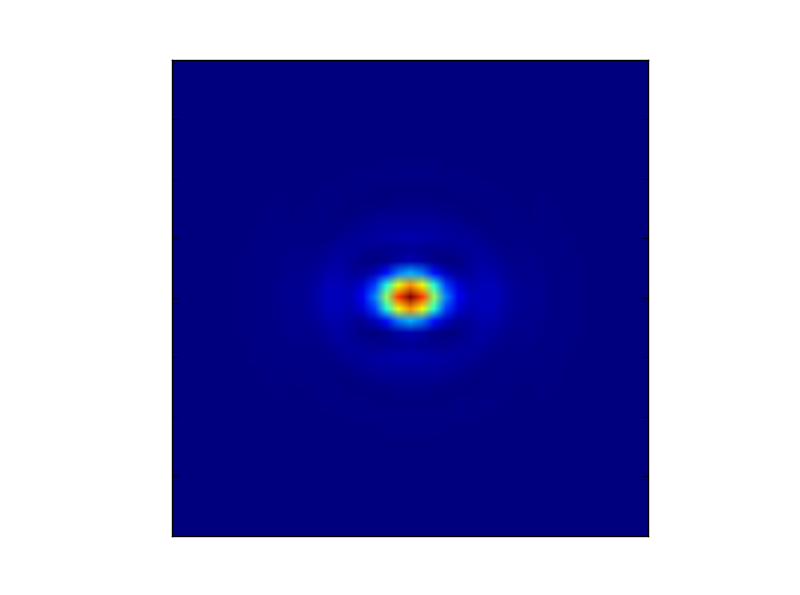
\includegraphics[width=\textwidth]{Figures/PSFzoomWthAb}
         \caption{PSF with aberrations ($a_j = 50 \mathrm{nm}$ for $a_{4}$, $a_{6}$and $a_{11}$, see subsec \ref{subsec:ZernikePol} for the definition of $a_j$, zoomed x10)}
         \label{subfig:PSFWthAb}
     \end{subfigure}
     \decoRule
     \caption{Comparison of perfect PSF and PSF with aberrations of an imaging system composed by a 3.6 mm pupil and a focal length of 80 mm at a wavelength of 637.5 nm. The size, N, of the PSF is 400 and the pixel size is 5.3 $\mu m$.}
     \label{fig:ComparisonPSFs}
 \end{figure} 

\subsection{Sources of aberration}
\label{subsec:SourcesAb}

The phase fluctuations introduced by aberrations are due to different kind of perturbation on the optical path. In ground based astronomy, the main source of aberrations is the \textbf{atmosphere}. Indeed, the atmosphere's temperatures fluctuations coupled with turbulent airflows are at the origin of the variations of the refractive index. Those variations induce then different optical path, in other words they generate perturbations on an electromagnetic wave passing through the atmosphere. The theory of the Atmospheric Turbulence is beyond the scope of this work, but we redirect the interested reader to \citet{obukhov1949,Tatarski1961,kolmogorov1968}.

The other source of aberrations are the \textbf{defects of the instrument} themselves. The defaults can limit the resolution and decrease the quality of an diffraction-limited imaging system. The defects can have multiple origins as described by \citet{Blanc2002}. The first one is a \textbf{default during the fabrication process}, such as mirror polishing. This kind of defect is fixed and of high spatial frequency. Perturbation of the electromagnetic wave can also be due to \textbf{misalignment of the optical components of the instrument}. For instance, during the first stages of operation stages of the Hubble telescope, the mirrors were not aligned and the resulting images were blurry. These defects are of low spatial frequency and vary slowly with time. Finally, there are defects due to \textbf{mechanical stresses of the instrument}. The mirrors have to be held in place by different mechanical components. And under the influence of the gravity, a mirror deformation can arise resulting in an aberration introduction. This kind of defect also evolves slowly through time but has a large spatial frequency domain.

In this work, we focus on a method to correct the effect of the instrument defects. This method is particularly suited since it does not require a different path than the path to the scientific instrument, which means that we can correct the aberrations on the entire optical path.

\subsection{Zernike polynomials}
\label{subsec:ZernikePol}

\begin{figure}
\begin{center}
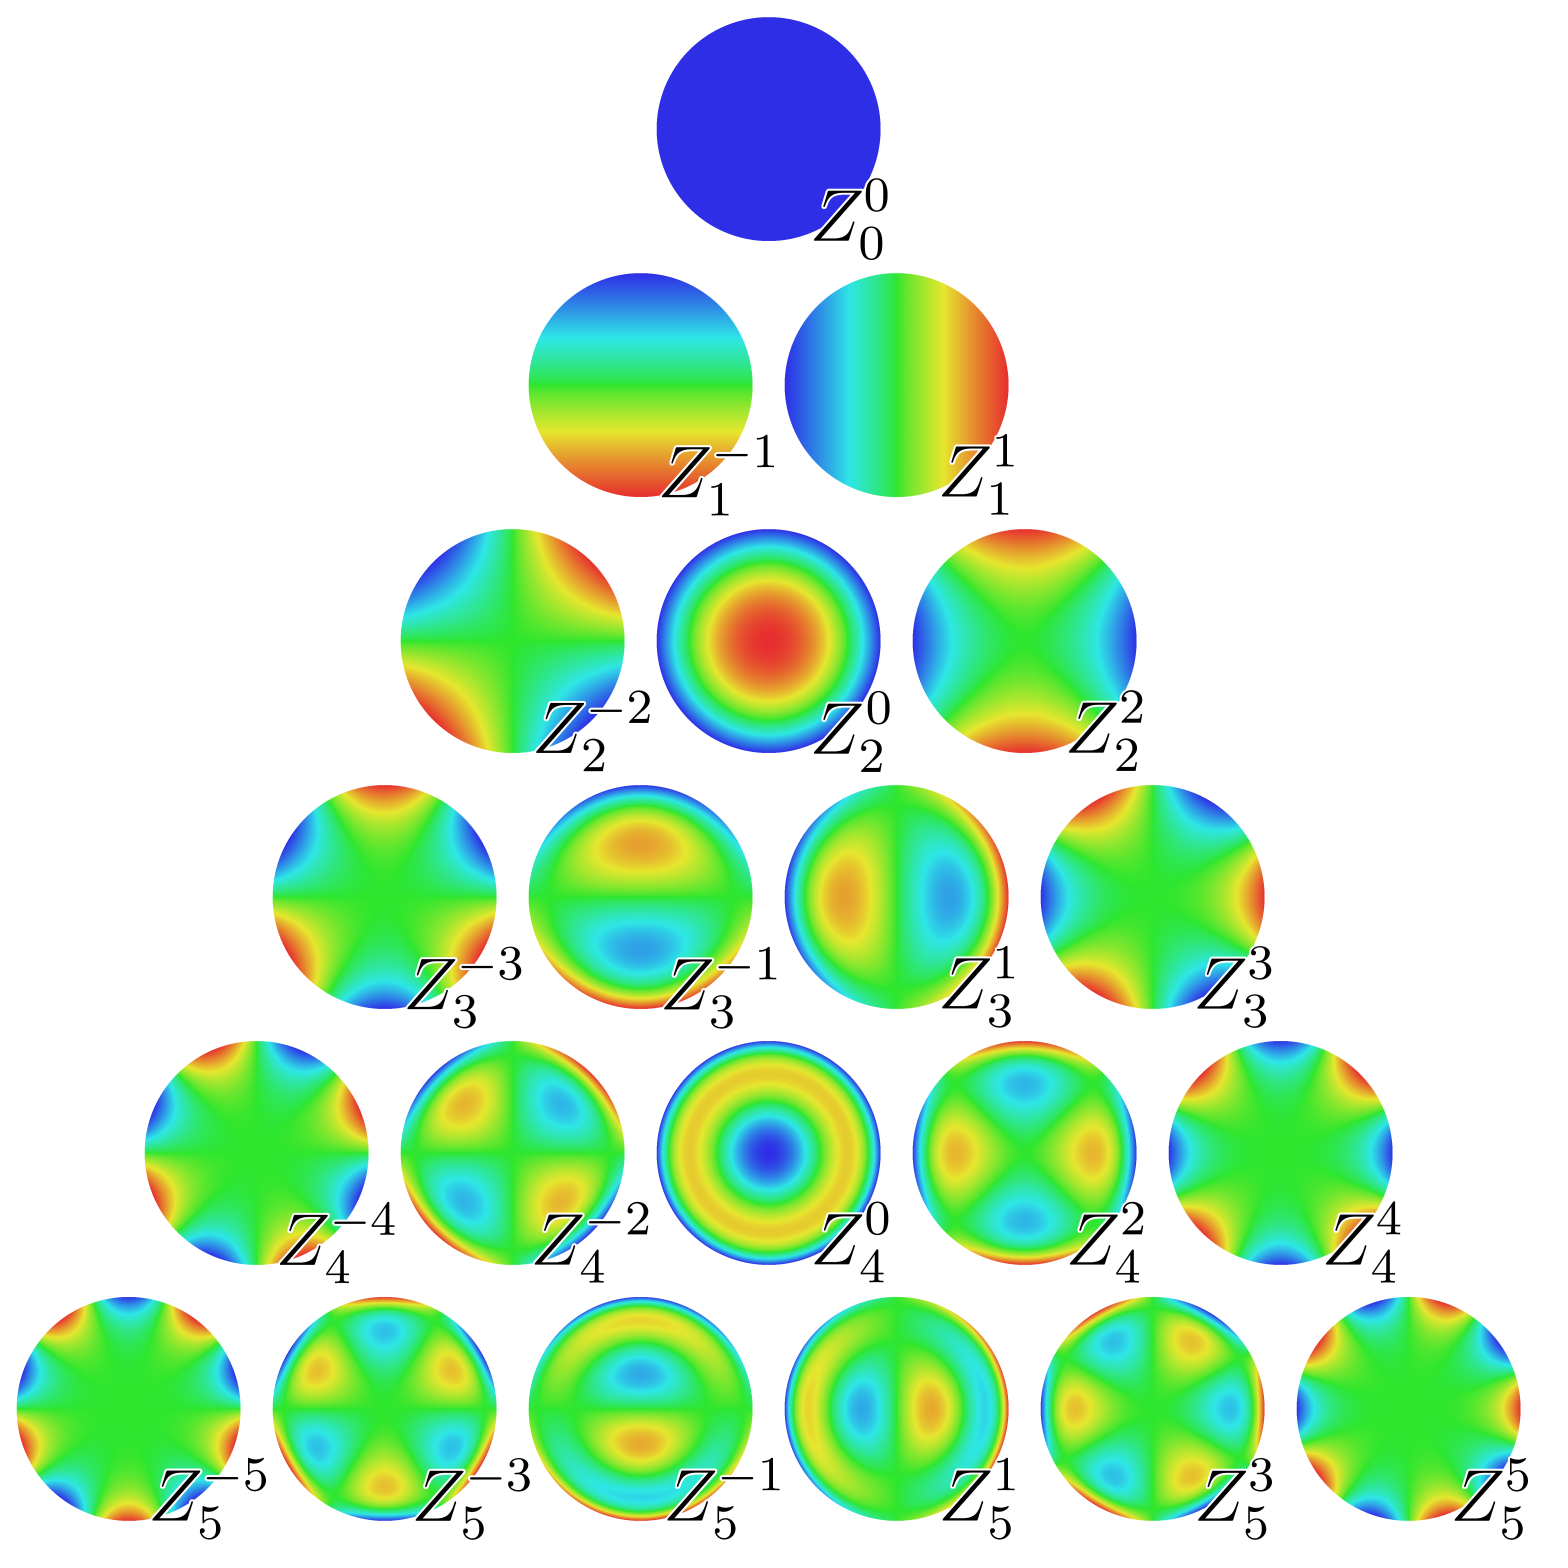
\includegraphics[width=\textwidth,angle=0]{Figures/Zernike_polynomials}
\decoRule
\caption[Representation of the 21$^{st}$ Zernike polynomials]{Representation of the 21$^{st}$ Zernike polynomials \citep{ZernikeWiki}}
\label{fig:Zernike_polynomials}
\end{center}
\end{figure}


In order to study the aberrations present in an imaging system, \citet{zernike1934} introduced an orthonormal basis on which we can decompose the phase on a circular pupil, such has a telescope pupil. Those polynomials are the factor of a trigonometric function and a polynomial function \citep{Noll_1976}.

\begin{equation}
Z_j(\mathbf{r}) = R_n^m(r)\Theta^m_n(\theta),
\label{eqt:ZernikePol}
\end{equation}

where $r=\frac{r'}{R_{pup}}$ is the normalized radius on the unit circle and $\theta$ is the azimuthal angle on the unit circle. $j$ correspond to the Zernike index in the Noll order, for a specific $j$ correspond only one couple $(n,m)$. The values of n and m are always integral and satisfy $|m| \leq n$, $n - |m| = \mathrm{even}$.

The trigonometric function is given by,

\begin{equation}
\Theta_n^m(\theta) = 
\begin{cases} 
\sqrt{n+1} &if m=0, \\
\sqrt{2(n+1)}cos(m\theta) &\mathrm{if} \ m \neq 0 \ \mathrm{and} \ i \ \mathrm{even}, \\
\sqrt{2(n+1)}sin(m\theta) &\mathrm{if} \ m \neq 0 \ \mathrm{and} \ i \ \mathrm{odd},
\end{cases}
\label{eqt:trigoFunc}
\end{equation}

and the radial function is given by,

\begin{equation}
R_n^m(r) = \sum\limits_{s=0}^{(n-m)/2}\frac{(-1)^s(n-s)!}{s![(n+m)/2-s]![(n-m)/2-s]!}r^{n-2s}.
\label{eqt:radialFunction}
\end{equation}

The decomposition of the phase onto the Zernike polynomials is given by,

\begin{equation}
\phi (\mathbf{r}) = \sum\limits_{i=1}^{+\infty}a_iZ_i(\mathbf{r}),
\label{eqt:decompPhase}
\end{equation}

where the $a_i$'s are the Zernike coefficient. And we characterize a wavefront by its root mean squared error without the piston component ($a_1$), which is given by,

\begin{equation}
\sigma_{\phi} = \sqrt{\frac{1}{S}\int\limits_S \phi^2(\mathbf{r})d\mathbf{r}} = \sqrt{\sum\limits_{i=2}^{+\infty}a_i^2},
\label{eqt:WFrmsError}
\end{equation}

where $S$ is the surface of the pupil.

\section{Phase retrieval}

The phase retrieval is a complicated process since the detectors are only sensitive to the intensity of a wave and not the wave itself, which renders impossible to have a direct relation between phase and image, thus we only have an indirect measurement of the wavefront. It is important to be able to estimate the aberrations of a system in order to correct them in real-time (Adaptive Optics systems) or in post-processing (Image restoration).

There are a couple of ways to characterize the form of a wavefront in order to determine the amplitude of the aberrations present in an imaging system. Some uses the optical geometric approximation, which says that locally the light rays are perpendicular to the wavefront. These achromatic methods measure the gradient of the wave surface, such as Shack-Hartmann \citep{hartmann1900,ShackPlatt_1971,fontanella1985}, Curvature sensing \citep{Roddier1988} and Pyramid sensing \citep{ragazzoni1996}. An other kind of methods are called interferometric or focal plane methods, they use the interference patterns of the pupil to determine the form of the wavefront. The Phase Diversity is part of those kind of methods, it was discovered by \citet{Gonsalves_1982}. The most popular method nowadays are the Shack-Hartmann, the curvature and the phase diversity. The latter will be explain in chapter \ref{ch:PDThe} and we will explain the principle of a Shack-Hartmann sensor since we will use it later on.


\subsection[Shack-Hartmann]{Shack-Hartmann \citep{hartmann1900,ShackPlatt_1971}}
\label{subsec:SHprinciple}

\begin{figure}
\begin{center}
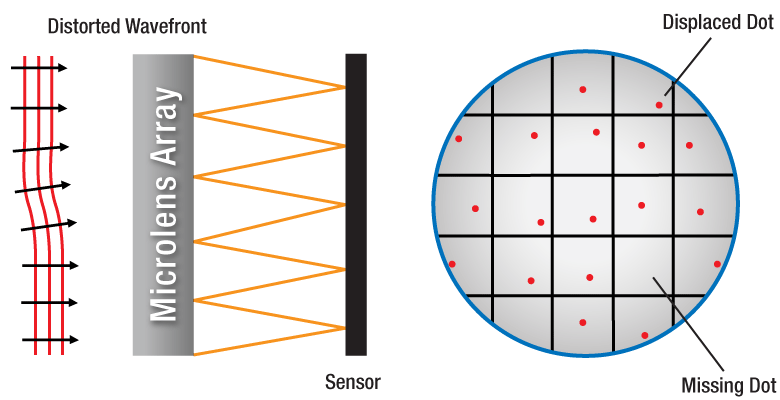
\includegraphics[width=\textwidth,angle=0]{Figures/SHWFSPrinciple}
\decoRule
\caption[Shack-Hartmann principle]{Shack-Hartmann principle \citep{SHWFS}}
\label{fig:SHWFSPrinciple}
\end{center}
\end{figure}

The Shack-Hartmann wavefront sensor measures the gradient of an aberrant phase. Figure \ref{fig:SHWFSPrinciple} shows the principle. A micro-lenses array samples the wavefront passing through the pupil in a conjugated plane of the entrance pupil. Each micro-lens produces a dot on a CCD placed at the focii of the micro-lenses. The deformations of the wavefront induce a displacement of the dot with respect to a reference position obtained with a perfectly planar or spherical wavefront. By measuring this displacement $\Delta x$, it gives directly the local slope of the wavefront \citep{fontanella1985},

\begin{equation}
\frac{2\pi}{\lambda}\frac{\Delta x}{f} = \frac{1}{S} \int\limits_S \frac{\delta\phi (x,y)}{\delta x}dxdy,
\label{eqt:SHWFSlope}
\end{equation}

where S is the surface of a micro-lens and f is the focal length of the micro-lenses. The wavefront is reconstructed by integrating over all the local slope measurements. The advantage of this technique is that it do not require a lot of computation since it is a direct measurement. But it requires an important optical system to acquire the data. It is used in many fields, especially in adaptive optics system to correct for the atmospheric turbulence.

